\chapter{Bibliotecas Digitais e Interoperabilidade}
\label{cap:bibinterop}
Nesse capitulo será apresentados conceitos sobre bibliotecas digitais, uma das soluções encontradas para catalogação dos mecanismos formais de participação.

\section{Conceitos Básicos Sobre Bibliotecas Digitais}

Uma biblioteca digital não é simplesmente uma coleção digital com ferramentas para manutenção das informações. Uma biblioteca digital é composta por um ambiente que possui coleções, serviços e pessoas apoiando um ciclo de vida de disseminação, uso e preservação do dado, informação e conhecimento.

De fato, as bibliotecas digitais vêm ganhando destaque por serem capazes de agregar valor aos serviços providos pelas bibliotecas tradicionais (não virtuais). Mediante o uso de protocolos que garantem interoperabilidade (como o Z39.50\footnote{Disponível em \url{http://pt.wikipedia.org/wiki/Z39.50}.} e o OAI-PMH\footnote{Informações disponíveis em \url{http://www.openarchives.org/}.}) e de padrões para descrição de metadados estruturais, descritivos, administrativos e de preservação \cite{rodrigrues2003preservacao}, as bibliotecas digitais tornaram-se suporte essencial para armazenamento, indexação, recuperação e distribuição de objetos digitais pela Internet. De acordo com a definição provida pela ARL\footnote{ARL ou Association of Research Libraries é uma organização composta por inúmeras instituições de pesquisa na área de Ciência da Informação – principalmente Estados Unidos e Canadá –, cujo objetivo é promover pesquisas, recomendar padrões e integrar as instituições envolvidas. Mais informações podem ser encontradas no endereço http://www.arl.org/.}, uma biblioteca digital é uma entidade que possui as seguintes características: (i) serve a vários usuários; (ii) é dirigida à tecnologia; (iii) é interligada com outras bibliotecas; (iv) é universalmente acessível; (v) não é limitada à digitalização de objetos impressos existentes; e (vi) pode ser provida de conteúdos multimídia que existam apenas em um ambiente digital.

Por sua vez, bibliotecas digitais não são apenas bibliotecas com conteúdo definido, mas entidades que têm uma variedade de propósitos e funções, dentre eles: (i) preservar objetos de informação; (ii) implantar melhorias na acessibilidade de materiais informacionais; (iii) integrar vários formatos de informação, sejam eles textuais, imagens e vídeos numa única coleção; e (iv) prover ferramentas de educação. 
Os objetos comportados em bibliotecas digitais representam artefatos que podem ou não terem sido captados do mundo real e existem modelos estabelecidos para a definição desses artefatos, como a proposição feita por \cite{kuramoto2007bibliotecas}, e que está ilustrada na figura \ref{fig:compartefdigital}.

Segundo \cite{arms2000digital}, ele ressalta que uma biblioteca digital é tão boa quanto assim for a sua interface, pois ela melhora a comunicação e reduz o esforço necessário para compreender a organização estrutural e espacial dos conteúdos, localizar objetos digitais específicos no sistema e nas telas, além de proporcionar uma navegação fácil. 

\graphicspath{{figuras/}}
\begin{figure}[H]
\centering
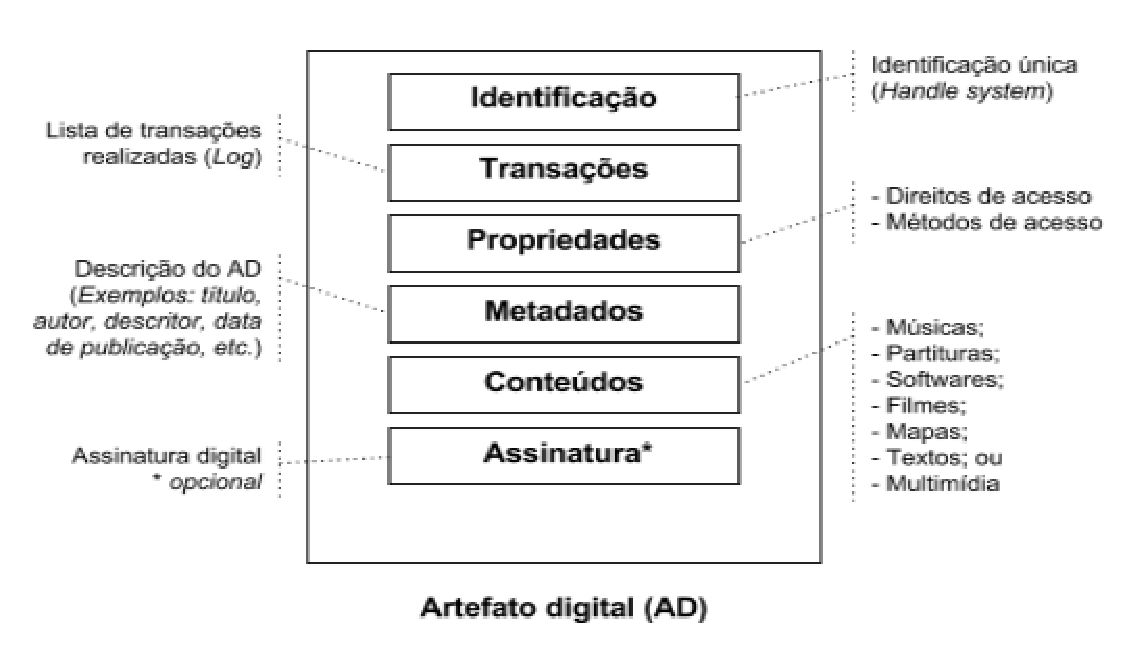
\includegraphics[width=0.8\textwidth]{artefato_digital}
\caption[Componentes de um artefato digital]{Componentes de um artefato digital. Adaptado de \cite{kuramoto2007bibliotecas}}
\label{fig:compartefdigital}
\end{figure}

Um objeto digital é a unidade básica de informação de uma biblioteca digital, em conjunto com os seus metadados e demais atributos, conforme está descrito na Figura \ref{fig:compartefdigital}.

Ainda de acordo com a figura \ref{fig:compartefdigital}, os artefatos digitais devem possuir: (i) uma assinatura digital como forma de certificação do produto; (ii) uma identificação do tipo de conteúdo que possui; (iii) os metadados descritivos, estruturais e administrativos; (iv) os direitos de acesso; (v) um controle de acessos e, finalmente (vi) uma identificação única. Abaixo é descrito cada um desses componentes: 

\begin{itemize}
	\item \textbf{Identificação} - Cada item tem que possui um identificador único, que é uma propriedade que distingue um objeto dos demais. Esse identificador pode ser um campo incremental, algum número de identificação único (CPF ou CNPJ), as iniciais do artefato (\textit{slugs}), entre outros.	
	\item \textbf{Transações} - É responsável por identificar e guardar em um arquivo de \textit{log} (registros), número de acessos a determinado artefato digital, quais itens do artefato digital foram acessados, etc.	
	\item \textbf{Propriedades} - Elas identificam quais são as diretivas de acesso para determinado artefato digital, no caso o artefato pode ser visualizado publicamente ou ter uma lista de determinados usuários que podem acessar o mesmo. Também identifica as  permissões de controle a esse item artefato (ler, editar, deletar). A propriedade identifica também qual será o caminho utilizado para se chegar a determinado artefato digital e como é feita a divisão do mesmo. Os métodos de acesso devem ser compatíveis com a forma de representação e devem atender a um público variado. Portanto, interfaces amigáveis (sistemas IHC – Interactive Human-Computer) para os diferentes tipos de usuário precisam ser contemplados.
	\item \textbf{Metadados} - Os metadados descrevem as características de um artefato digital \footnote{Visto mais detalhadamente adianta, na seção \ref{sec:padraometadado}}.	
	\item \textbf{Conteúdo} - O conteúdo é algo que faz parte de um artefato digital. Um artefato digital pode ser composto de vários tipos de conteúdo (áudio, vídeo, imagem, textos, etc.). 	
	\item \textbf{Assinatura} - A assinatura digital garante a autenticidade daquele artefato digital. Ele garante que o item acessado possui veracidade em suas informações, além de garantir também que as informações acessadas pelo usuários são integras (nada foi perdido).
\end{itemize}

Para uma prova de conceito da versão da biblioteca digital do Participa.br que será vista na subseção \ref{sub:prototipo_biblioteca}, a identificação é composta por um campo que auto incrementa a cada novo canal de participação cadastrado. As transações são compostas pelos \textit{logs} de acesso do próprio apache, que fornece os dados de acesso dos usuários \footnote{Os \textit{logs} do \textit{Apache} não fornece detalhes sobre os acessos sobre cada artefato digital, isso será implementado}. As propriedades de acesso definidas para os itens são (i) público - qualquer usuário pode acessar o item e (ii) privada - somente usuários permitidos em uma lista podem acessar o item.

Os Metadados serão explicados na subseção \ref{sub:metadadospbr}, onde será feita uma relação com os metadados DC, com os metadados do Participa.br. Em relação ao tipo de conteúdo, somente os no formato de texto digital(HMTL, TXT e PDF) foram relevados, no entanto, já foi levantado que existem conselhos e conferências que disponibilizam vídeos e áudios de suas reuniões. A assinatura digital não foi disponibilizada nessa primeira prova de conceito, já que serão feitas futuras reuniões com os gestores da SGPR com vistas de verificar a necessidade de implementação de assinaturas.

De acordo com o que está apresentado na figura \ref{fig:modelbibdigital}, o projeto de interface é parte integrante do modelo conceitual do sistema, juntamente com o projeto funcional que especifica as funções a serem oferecidas aos usuários e ao projeto dos metadados associados aos dados que especificam a estrutura e a organização e descrição do conteúdo \cite[pp. 143--145]{arms2000digital}\cite[pp. 190]{ferreira2006interface}.

\graphicspath{{figuras/}}
\begin{figure}[H]
\centering
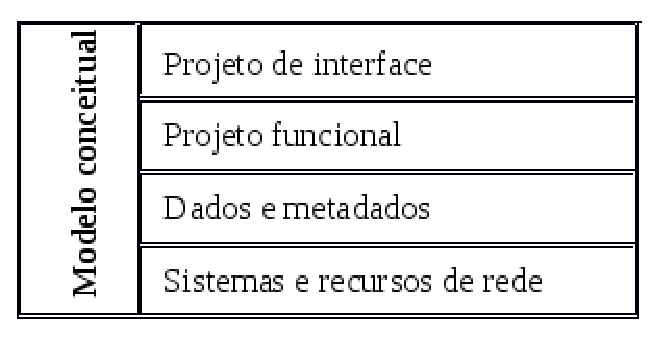
\includegraphics[width=0.5\textwidth]{modelo_biblioteca}
\caption[Modelo conceitual para projeto de bibliotecas digitais]{Modelo conceitual para projeto de bibliotecas digitais. Extraído de \cite[p. 144]{arms2000digital}}
\label{fig:modelbibdigital}
\end{figure}

Para o caso dos canais de participação social, esse modelo também pode ser usado como referência, dada a variedade de possibilidades de acesso, tipos de usuários e formas de representação dos artefatos digitais. Tais possibilidades impactam diretamente na construção das interfaces de acesso, dando origem a paradigmas que permitem expressões de busca diferenciadas.

Ainda de acordo com esse o modelo ilustrado pela figura \ref{fig:modelbibdigital} faz-se necessário implementar uma biblioteca completa, com os sistemas (busca, navegação, catalogação e demais) totalmente integrados, isso ajuda os usuários com uma biblioteca mais harmônica e robusta, consequentemente, tendo uma confiança na utilização da biblioteca pelo usuário. As figuras \ref{fig:sistemasoftware}  e \ref{fig:entregaveissoftware}

\graphicspath{{figuras/}}
\begin{figure}[H]
\centering
\includegraphics[width=0.8\textwidth]{sistemas}
\caption[Identificação dos principais componentes de uma biblioteca]{Identificação dos principais componentes de um site. Adaptado de \cite{rosenfeld2002information}}
\label{fig:sistemasoftware}
\end{figure}

De acordo com a figura, para melhor entendimento de uma biblioteca digital é necessário entregar um detalhamento maior das arquiteturas que compõe a mesma, isso facilita a interação do usuário com a biblioteca. Um sistema de busca não é composto somente por uma interface bonita ou um bom motor de busca, mas por todo um conjunto integrado. O usuário tem que ser capaz de pesquisar qualquer tipo de conteúdo e ordena-lo de forma que achar melhor e os resultados precisam ser apresentados de forma satisfatória. Para isso é necessário catalogar os artefatos digitais, pois isso ajuda na indexação da pesquisa, assim como ampliar o sistema para permitir o vocabulário semântico. Também é necessário planejar o esquema de navegação da biblioteca, deixando os menus organizados para que facilite a utilização do site pelo usuário.

\graphicspath{{figuras/}}
\begin{figure}[H]
\centering
\includegraphics[width=0.8\textwidth]{entregaveis}
\caption[Entregáveis de uma biblioteca]{Entregáveis de uma biblioteca. Adaptado de \cite{rosenfeld2002information}}
\label{fig:entregaveissoftware}
\end{figure}

A figura \ref{fig:entregaveissoftware} mostra os entregáveis de uma biblioteca, são utilizados para um entendimento melhor do sistema a ser produzido. Os \textit{Blueprints}, também chamados de mapa do site são uma espécie do funcionamento de toda a arquitetura de informação presente no site. Eles mostram as relações de caminho entres as páginas e seus componentes. Os Wireframes descrevem uma página individual, mostrando todos os conteúdos e arquitetura da informação relacionados com a página através de um protótipo. Esse protótipo pode dizer quais informações podem ser informadas para o usuário e servir de insumo para o sistema final. Os vocabulários controlados permitem que um item seja encontrado através de palavras relacionadas, isso ajuda o cliente em interfaces de busca. Um exemplo de vocabulário controlado é um tesauro \footnote{Maiores informações em: \url{http://pt.wikipedia.org/wiki/Tesauro}}. O esquema de metadados, explicado mais detalhadamente na seção \ref{sec:padraometadado} ajudam a catalogar melhor os objetos digitais, fazendo com que a indexação de busca seja melhor.

Nesse primeiro trabalho, foram levantados alguns metadados com base no catálogo de mecanismos formais, disponível no Anexo \ref{Att:catalogomecanismos}. O produto de cada catalogação gerou um primeira versão do esquema de metadados, que é visto na seção \reflabel{sub:metadadospbr}. Apesar de não ser necessariamente um Wireframe, o primeiro protótipo da biblioteca digital de participação social visto na seção \ref{sub:prototipo_biblioteca} pode ser entendido como um, já que apresenta uma interface inicial onde há a exibição de conteúdos para os usuários.

\section{Padrões de metadados para catalogação e sistematização de dados}
\label{sec:padraometadado}

Na biblioteconomia, o metadado é dado estruturado que compartilha diversas características similares para a catalogação e descrevem as características de um determinado recurso informacional. Um registro de metadados consiste em um número predefinido de elementos que representam atributos específicos de um objeto e cada elemento pode estar associado a um ou mais valores. Os esquemas de metadados devem possuir (independente da área de conhecimento) um número limitado de elementos, o nome de cada elemento e o significado de cada elemento.

Dentre os benefícios de metadados na web, pode-se citar os seguintes: (i) são estruturados e formam a base para o desenvolvimento de sistemas de busca, (ii) podem ser convertidos para outros formatos, ou seja, interoperar com diferentes protocolos de busca e recuperação, (iii) tornam mais fácil a extração de conteúdo por engines de busca (SEOs) e (iv) facilitam o gerenciamento do sistema de informação (com os metadados administrativos) porque ajudam a avaliar quando os recursos devem ser revistos ou removidos da base de dados.

Em relação agrupamento dos elementos de metadados de um recursos computacional (classificação), podem ser classificados em:

\begin{itemize}
	\item \textbf{Descritivos} Passíveis de uso por sistemas de busca. Por exemplo o título, a descrição, URI, autor, idioma, formato de arquivo;
	\item \textbf{De assunto} (Relacionados à atividade de indexação) descrevem o conteúdo do documento, tais como as palavras-chave, os códigos e sistemas de classificação, termos do tesauro ou cabeçalho de assuntos; e
	\item \textbf{Administrativos} que facilitam a organização e administração do sistema de informação. Exemplos incluem o responsável pela manutenção do documento, data de adição do documento, data de expiração, dentre outros.
\end{itemize}

Do ponto de vista do grau de dificuldade de uso dos padrões, os metadados, podem ser classificados em formatos de bandas um, dois e três \cite{feitosa2006organizacao}. Os formatos de metadados de banda um envolvem a indexação automática de texto integral, e em geral é feito por softwares proprietários, portanto não acessíveis para manipulação.

Os formatos de banda dois permitem a descrição que não exige grande especialidade para sua aplicação enquanto os formatos de banda três são aqueles que provêem uma descrição mais especializada, geralmente descrita segundo padrões estabelecidos, como o AACR2 (vide exemplo na figura \ref{fig:aacr2}). 

\graphicspath{{figuras/}}
\begin{figure}[H]
\centering
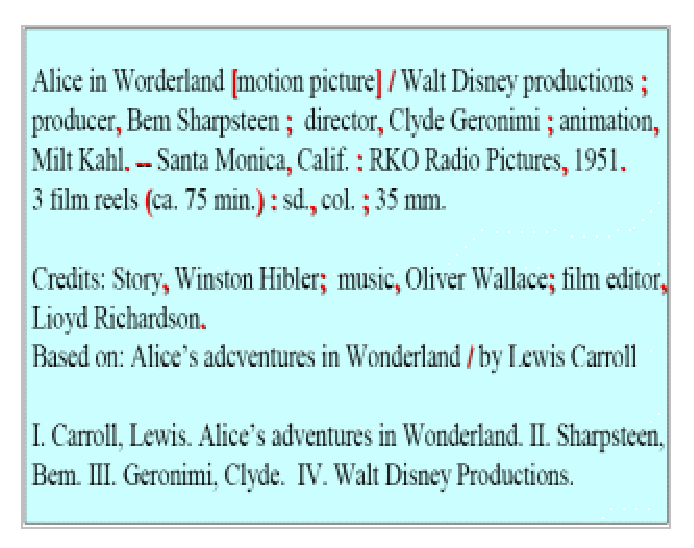
\includegraphics[width=0.7\textwidth]{aacr2}
\caption{Ficha catalográfica considerando as recomendações AACR2}
\label{fig:aacr2}
\end{figure}

Percebe-se que as descrições são para especialistas na área de catalogação e são feitas com domínio sobre os formatos e sobre as regras de classificação associadas. Um exemplo de catalogação na banda três está apresentado na figura \ref{fig:marc2}, com a descrição de um registro no formato MARC, de uso comum por profissionais da área da Biblioteconomia.

\graphicspath{{figuras/}}
\begin{figure}[H]
\centering
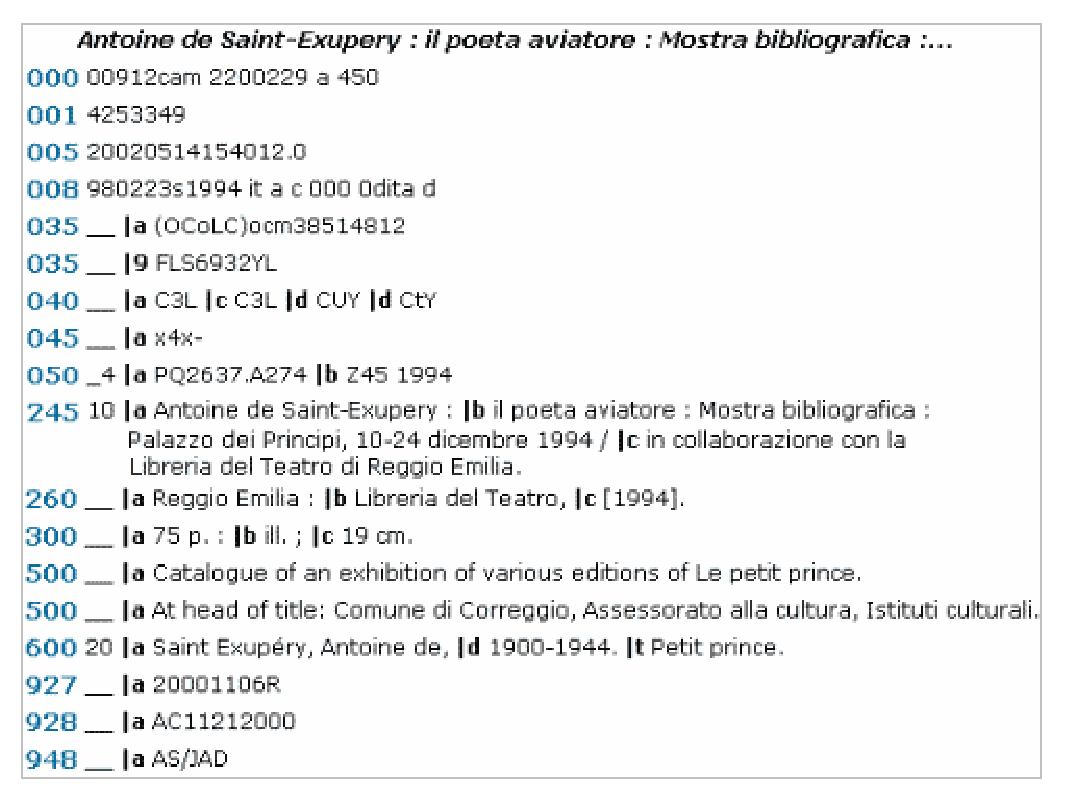
\includegraphics[width=0.7\textwidth]{marc2}
\caption{Exemplo de descrição bibliográfica em formato MARC}
\label{fig:marc2}
\end{figure}

Em função das características citadas, para o catalogação dos dados do Participa.br sugere-se a utilização dos formatos de banda 2, mais especificamente o Dublin Core, que deve ser tomado como referência para criação de qualificadores para os conteúdos de participação social. O Dublin Core é interessante porque envolve um conjunto de dados padronizados para descrição de recursos na web. Caracteriza-se por sua utilidade e flexibilidade na representação dos dados e contém 15 elementos na sua composição básica, conforme exemplo descrito na figura \ref{fig:exdublincore}. Esse padrão é acordo conceitual sobre termos de fácil uso e não necessita ser especializado no processo de catalogação para descrição dos recursos na web.

\graphicspath{{figuras/}}
\begin{figure}[H]
\centering
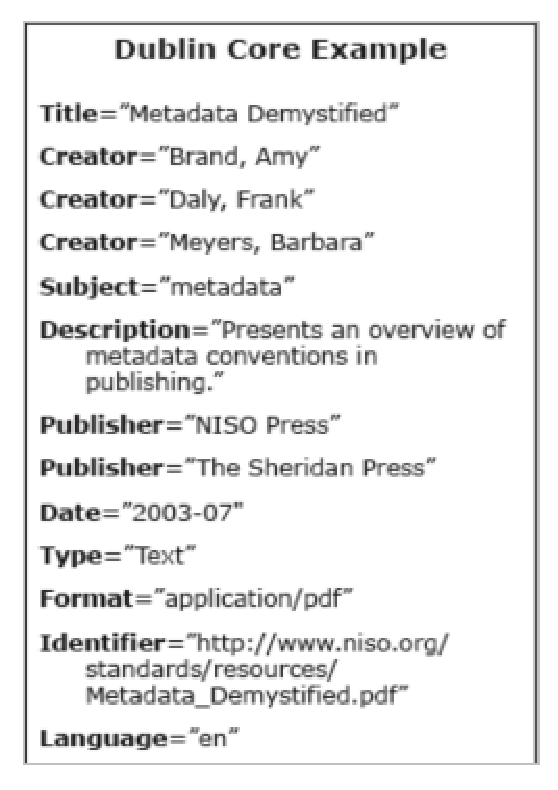
\includegraphics[width=0.5\textwidth]{exemplo_dublincore}
\caption{Exemplo de escrição bibliográfica em formato Dublin Core}
\label{fig:exdublincore}
\end{figure}



